\chapter{Graph Theory}
\label{chp:graph-theory}
In this chapter we will provide the fundamentals of the graph theory concepts required to understand the rest of the thesis. In Section~\ref{sec:prelim} we cover the basic definitions, terminologies used to describe different types of graphs. Then we define a signed graph and discuss its unique properties in Section~\ref{sec:signed-graphs}. We outline the theory of balance in signed networks and methods to measure it in Section~\ref{sec:balance-theory}.Next, we discuss the theory of status and illustrate the differences to balance in Section~\ref{sec:status-theory}. Lastly, we explain techniques of finding hierarchies in directed networks and the concept of agony in Section~\ref{sec:hierarchy}.

\section{Preliminaries}
\label{sec:prelim}
In this section we define the various types of graphs and their basic properties. The notation and terminologies used closely follows those used in Diestel~\cite{diestel1997graph}. Graphs are structures that describe relationships between entities. These entities are called \textit{vertices} and entities related to one another are joined by edges. The terms graph, vertices and edges can be used interchangeably with \textit{network}, \textit{nodes} and \textit{links} respectively.

Graphs can be classified broadly into two types based on whether the edges posses a direction or not. We now go on to define them in detail.
\subsection{Undirected Graphs}
An undirected graph is pair $G=(V,E)$, where $V$ is the set of vertices and $E$ is the set $E \subseteq \{ (u,v) \mid u,v \in V\}$ of unordered pairs of vertices called edges. In this thesis we will deal with only \textit{simple graphs}, i.e. no are so self loops $(u,v)\in V \times V, ~ u\neq v$ and there is at most one edge between vertices $u$ and $v$. 

The number of the vertices in a graph is called the \textit{order} of the graphs is denoted by $n= |G|$ and the \textit{size} of a graph is the number of edges denoted by $m = \|G\|$ or $m=|E|$. A vertex $u$ is \textit{adjacent} to $v$ is they are the end points of an edge, $(u,v) \in E$. All the vertices adjacent to vertex $v$ is called the \textit{neighbourhood} of $v$ and is denoted by $N(v)$. The \textit{degree} of a vertex $v$ is the number of nodes adjacent to that vertex and is denoted by $d(v) = |N(v)|$. 

The edges of an undirected graph can also have an associated value. This value can indicate the distance or similarity between a pair of vertices. These values are called \textit{weights} and the corresponding graph is called a \textit{weighted undirected graph}. Therefore, a weighted graph is defined as a triple $G=(V,E,w)$, where $w:E \rightarrow \mathbb{R}^{+}$ is a function that maps an edge $e$ to a positive real weight $w(e)$. Now an \textit{unweighed graph} is simply a weighted graph where the function $w$ is defined as: if $e \in E$ then $w(e)=1$ else $w(e)=0$. The degree of a a vertex $v$ in a weighed graph is the sum of the weights to all the neighbours of $v$ and is defined as $d(v) = \sum_{u\in N(v)}w((u,v))$ An example of a weighted undirected graph is shown in Figure~\ref{fig:weighted-undirected}. 
\begin{figure}[!ht]
    \centering
    \tikzset{
    position/.style args={#1:#2 from #3}{
        at=(#3.#1), anchor=#1+180, shift=(#1:#2)
    }
}

\begin{tikzpicture}

    \begin{scope}[every node/.style={circle,thick,draw}]
        \node (v1) at (0,0) {$v_1$};
        \node[below=1cm of v1] (v2) {$v_2$};
        \node[position=45:2cm from v2] (v3) {$v_3$};
        \node[position=150:2cm from v1] (v4) {$v_4$};
        \node[left=3cm of v2] (v5) {$v_5$};
        \node[position=45:1cm from v5] (v6) {$v_6$};
    \end{scope}

    \begin{scope}[>={Stealth[red]},
        every edge/.style={thick,draw},
        every node/.style={fill=white,circle}]
        % \draw (v4) -- (v1) -- (v3) -- (v2) -- (v1);
        \path (v1) edge (v2) 
            (v2) edge (v3)
            (v1) edge node[above] {$1$} (v3)
            (v1) edge (v4)
            (v5) edge (v6)
            ;
    \end{scope}
  \end{tikzpicture}
  
    \caption{An example of a weighted undirected graph}
    \label{fig:weighted-undirected}
\end{figure}


\subsection{Directed Graphs}
The main distinction regarding a \textit{directed graph} (or \textit{digraph}) is that the edges are ordered pairs, i.e.$(u,v) \neq (v,u)$. Therefore, a directed graph has a similar definition: a pair $G=(V,E)$, where $V$ is the set of vertices and $E$ is the set of \textit{ordered} pairs of vertices. Now given an edge $e=(u,v)$ we can define a source function $\src:E\rightarrow V$ such that $\src(e)=u$ and a destination function $d:E\rightarrow V$ where $\dest(e)=v$. These functions classify the vertices in an edge $e$ as either the source or the destination. In this thesis, we deal only with \textit{simple directed graphs}, i.e. no self-loops and there can be at most one edge from $u$ to $v$. 

As the edges now have an inherent direction we can define the \textit{successors} and \textit{predecessors} of a node $v$. A vertex $u$ is called the \textit{successor} of a node $v$ is there exists a directed edge from $v$ to $u$, therefore the set of successors for a vertex $v$ can be defined as $S(v) = \{u \mid (v,u) \in E\}$. A \textit{predecessor} of a node $v$ is a vertex $u$ such that there exists a directed edge from $u$ to $v$, the set of predecessors for a vertex $v$ can de defined as $P(v) = \{u \mid (u,v) \in E\}$. We now a vertex $u$ that is either a successor or a predecessor of a vertex $v$ can be called a neighbour of the vertex $v$. Therefore, we define the \textit{neighbourhood} of a vertex $v$ as the set of vertices in the union of successors and predecessor, i.e $N(v) = S(u) \cup P(v)$. This definition is also compatible with undirected graphs because if $(u,v) \in E$ then $(v,u) \in E$. 

Directed graphs can also have values associated with each directed edge called a \textit{weight}. A \textit{weighted directed graph} can be defined as a triple $G=(V,E,w)$, where the weight function $w:E \rightarrow \mathbb{R}^{+}$ that maps each edge $e$ to a weight $w(e)$. The indegree of a vertex $v$ is defined as the sum of the edge weights from the predecessors of $v$ and is denoted as $\indegree(v) = \sum_{u \in P(v)} w((u,v))$. Similarly, the outdegree of a vertex $v$ is defined as the sum of the edge weights to the successors of $v$ and is denoted by $\outdegree(v) = \sum_{u \in S(v)}w((v,u))$.
Figure~\ref{fig:weighted-directed} shows an example of a weighted directed graph.

\begin{figure}[!ht]
    \centering
    \tikzset{
    position/.style args={#1:#2 from #3}{
        at=(#3.#1), anchor=#1+180, shift=(#1:#2)
    }
}

\begin{tikzpicture}

    \begin{scope}[every node/.style={circle,thick,draw}]
        \node (v1) at (0,0) {$v_1$};
        \node[below=2cm of v1] (v2) {$v_2$};
        \node[right=2cm of v2] (v3) {$v_3$};
        \node[above=2cm of v3] (v4) {$v_4$};
        \node[below right=1cm and 2cm of v4] (v5) {$v_5$};
        \node[below left=1cm and 2cm of v1] (v6) {$v_6$};
    \end{scope}

    \begin{scope}[>={Stealth[black]},
        every edge/.style={thick,draw},
        every node/.style={fill=white,circle}]
        % \draw (v4) -- (v1) -- (v3) -- (v2) -- (v1);
        \path[->] 
        (v1) edge[bend right=20] node[left] {$2$} (v2)
        (v2) edge[bend right=30] node[below right=1mm] {$4$} (v4)  
        (v1) edge[bend left=35] node[above=0.8mm] {$1$} (v4)
        (v4) edge[bend left=35] node[below=0.8mm] {$1.5$} (v1)
        (v5) edge[bend left=30] node[below right=1mm] {$3.5$} (v3)
        (v2) edge[bend left=30] node[below left=0.8mm and 0.8mm] {$2.5$} (v6)
        ;
    \end{scope}
  \end{tikzpicture}
  
    \caption{An example of a weighted directed graph}
    \label{fig:weighted-directed}
\end{figure}

\section{Signed Graphs}
\label{sec:signed-graphs}
The simple weighted graphs we have defined so far only have non-negative edge weights that can represent similarity or closeness. In the 1950s social psychologists found it desirable to express liking, disliking or indifference in social interactions. This was formalized by Harary \cite{harary1953on} using graphs with weights $(-1,0,1)$. These graphs are therefore called \textit{signed graphs}, where a negative edge weight can denote dissimilarity between a pair of vertices. In this thesis we will use notations and terms similar to Gallier \cite{gallier2016spectral}, Kunegis et al. \cite{kunegis2010spectral}, Hou \cite{hou2005bounds} and Zaslavsky \cite{zaslavsky1982signed}.

A signed graph is a triple $G=(V,E,w)$, where $V$ is the set of vertices, $E$ is the set of pair of vertices and the weight function $w:E \rightarrow \mathbb{R}$. The weight function now takes an edge $e$ and maps it to a signed weight $w(e)$. We can partition the edges into positive and negative edges, $E = E^{+}\cup E^{-}$, where $E^{+} = \{e \mid w(e)>0\}$ and $E^{-}=\{e \mid w(e)<0\}$. Similar to Zaslavsky \cite{zaslavsky1982signed}, we consider undirected signed graphs and directed signed graphs as distinct and separate entities. We can see some examples of signed graphs in Figure~\ref{fig:signed-graphs}.
\begin{figure}[!ht]
    \centering
    \begin{subfigure}{0.5\textwidth}
        \centering
        \tikzset{
    position/.style args={#1:#2 from #3}{
        at=(#3.#1), anchor=#1+180, shift=(#1:#2)
    }
}

\begin{tikzpicture}

    \begin{scope}[every node/.style={circle,thick,draw}]
        \node (v1) at (0,0) {$v_1$};
        \node[below=1cm of v1] (v2) {$v_2$};
        \node[position=45:2cm from v2] (v3) {$v_3$};
        \node[position=150:2cm from v1] (v4) {$v_4$};
        \node[left=3cm of v2] (v5) {$v_5$};
        \node[position=45:1.3cm from v5] (v6) {$v_6$};
    \end{scope}

    \begin{scope}[>={Stealth[red]},
        every edge/.style={thick,draw},
        every node/.style={fill=white,rectangle}]
        % \draw (v4) -- (v1) -- (v3) -- (v2) -- (v1);
        \path (v1) edge node[left] {$2$} (v2) 
            (v2) edge node[below right=0.05cm and 0.05cm] {$-1.5$} (v3)
            (v1) edge node[above=0.05cm] {$-1$} (v3)
            (v1) edge node[above right] {$4$} (v4)
            (v5) edge node[above left] {$-3$} (v6)
            ;
    \end{scope}
  \end{tikzpicture}
  
        \caption{A undirected signed graph}
        \label{fig:signed-undirected}
    \end{subfigure}

    \begin{subfigure}{0.5\textwidth}
        \centering
        \tikzset{
    position/.style args={#1:#2 from #3}{
        at=(#3.#1), anchor=#1+180, shift=(#1:#2)
    }
}

\begin{tikzpicture}

    \begin{scope}[every node/.style={circle,thick,draw}]
        \node (v1) at (0,0) {$v_1$};
        \node[below=2cm of v1] (v2) {$v_2$};
        \node[right=2cm of v2] (v3) {$v_3$};
        \node[above=2cm of v3] (v4) {$v_4$};
        \node[below right=1cm and 2cm of v4] (v5) {$v_5$};
        \node[below left=1cm and 2cm of v1] (v6) {$v_6$};
    \end{scope}

    \begin{scope}[>={Stealth[black]},
        every edge/.style={thick,draw},
        every node/.style={fill=white,rectangle}]
        % \draw (v4) -- (v1) -- (v3) -- (v2) -- (v1);
        \path[->] 
        (v1) edge[bend right=20] node[left=0.05cm] {$-2$} (v2)
        (v2) edge[bend right=30] node[below right=1mm] {$4$} (v4)  
        (v1) edge[bend left=35] node[above=0.8mm] {$-1$} (v4)
        (v4) edge[bend left=35] node[below=0.8mm] {$1.5$} (v1)
        (v5) edge[bend left=30] node[below right=1mm] {$3.5$} (v3)
        (v2) edge[bend left=30] node[below left=0.8mm and 0.8mm] {$2.5$} (v6)
        ;
    \end{scope}
  \end{tikzpicture}
  
        \caption{A directed signed graph}
        \label{fig:signed-directed graph}
    \end{subfigure}
    \caption{Examples of Signed Graphs}
    \label{fig:signed-graphs}
\end{figure}

We can now proceed to define a few more terms. The degree of a vertex $v$ is now the sum of the absolute edge weight of its neighbours is called the \textit{signed degree} and is defined as 
\[
    \overline{d}(v) = \sum_{u \in N(v)}|w((u,v))|
\] 
This can also be extended to \textit{signed indegree} and \textit{signed outdegree} denoted by $\overline{\indegree}(v)$ and $\overline{\outdegree}(v)$ and defined as
\[
    \overline{\indegree}(v)=\sum_{u \in P(v)}|w((u,v))|
\] 
\[
    \overline{\outdegree}(v)=\sum_{u \in S(v)}|w((v,u))|
\] 

We can create a $n \times n$ square weight matrix $W$, where each entry $w_{ij}$ is defined as 

\[ w_{ij} = 
\begin{cases}
    w((v_i,v_j)) & \text{if } (v_i,v_j) \in E \\
    0 & \text{if } (v_i,v_j) \notin E      
\end{cases}
\] 
The signed degree matrix $\overline{D}$ is a diagonal matrix consisting of the signed verted degrees, $\overline{D} = \text{diag}(\overline{d}(v_{1}),\dots,d(v_n))$. We can now define the \textit{signed Laplacian}, $\overline{L}$ as 
\[ \overline{L} = \overline{D} - W\]
The signed Laplacian along with results from spectral analysis of signed graphs \cite{hou2005bounds,kunegis2010spectral}, will be useful for balance theory of signed graphs. 

\subsection{Balance Theory}
\label{sec:balance-theory}


Heider \cite{heider1946attitudes} proposed in 1940's that when there are either \textit{positive relations} (friendship, love, support) and \textit{negative relations} (enmity, hate, oppose) in a group, the  group tends towards \textit{balance}. Balance was defined as there being all positive relations or one positive and two negative relations for a group of 3 people. Harary and Cartwright \cite{cartwright1956structural} generalized this notion of balance by using signed graphs. As these relations are typically symmetric, balance is usually defined for undirected signed graphs. This can been seen in Figure~\ref{fig:signed-triads} where solid edges are positive and dashed edges are negative. Social psychology also showed that balanced triads $B_1$ and $B_2$ mirror aphorisms such as "the friend of my friend is also a friend" and "the enemy of my enemy is a friend" respectively.

\begin{figure}[!ht]     
    \centering
    \tikzset{
    position/.style args={#1:#2 from #3}{
        at=(#3.#1), anchor=#1+180, shift=(#1:#2)
    }
}

\begin{tikzpicture}

    \begin{scope}[every node/.style={circle,thick,draw}]
        \node (v1) at (0,0) {};
        \node[position=-120:1cm from v1] (v2) {};
        \node[position=-60:1cm from v1] (v3) {};
        
        \node[right=2cm of v1] (v4) {};
        \node[position=-120:1cm from v4] (v5) {};
        \node[position=-60:1cm from v4] (v6) {};
        
        \node[right=2cm of v4] (v7) {};
        \node[position=-120:1cm from v7] (v8) {};
        \node[position=-60:1cm from v7] (v9) {};
        
        \node[right=2cm of v7] (v10) {};
        \node[position=-120:1cm from v10] (v11) {};
        \node[position=-60:1cm from v10] (v12) {};
        

    \end{scope}

    \begin{scope}[>={Stealth[red]},
        positive/.style={thick,draw},
        negative/.style={thick,dashed,draw},
        every node/.style={fill=white,circle}]
        % \draw (v4) -- (v1) -- (v3) -- (v2) -- (v1);
        \path 
        (v1) edge[positive] node[above left=0.1mm and 0.1mm] {$+$} (v2)
        (v1) edge[positive] node[above right=0.1mm and 0.1mm] {$+$} (v3) 
        (v3) edge[positive] node[below] {$+$} node[below=1cm] {$T_1$}  (v2)      
        ;
        \path 
        (v4) edge[negative] node[above left=0.1mm and 0.1mm] {$-$} (v5)
        (v4) edge[negative] node[above right=0.1mm and 0.1mm] {$-$} (v6) 
        (v6) edge[positive] node[below] {$+$} node[below=1cm] {$T_2$}  (v5)      
        ;
        \path 
        (v7) edge[positive] node[above left=0.1mm and 0.1mm] {$+$} (v8)
        (v7) edge[positive] node[above right=0.1mm and 0.1mm] {$+$} (v9) 
        (v9) edge[negative] node[below] {$-$} node[below=1cm] {$T_3$}  (v8)      
        ;
        \path 
        (v10) edge[negative] node[above left=0.1mm and 0.1mm] {$-$} (v11)
        (v10) edge[negative] node[above right=0.1mm and 0.1mm] {$-$} (v12) 
        (v12) edge[negative] node[below] {$-$} node[below=1cm] {$T_4$}  (v11)      
        ;
    \end{scope}
  \end{tikzpicture}
    
    \caption{Triads in undirected signed graphs. $B_1$ and $B_2$ are \textit{balanced} triads as they have even number of negative edges. $B_3$ and $B_4$ are \textit{unbalanced} as they have odd number of negative edges.}
    \label{fig:signed-triads}
\end{figure}

The concept of balance can be generalized to state that an undirected signed graph $G=(V,E,w)$ is balanced iff every cycle in $G$ has an even number of negative edges. This leads to result from Harary \cite{harary1953on} that states that if a graph $G$ is balanced, then there is a partition of the vertices $V = V_1 \cup V_2$ such that edges within the vertices of each set is positive and edges between the sets are negative. This means that we can have a bipartite graph when we delete the positive edges and negative edges span between the two sets of vertices. An example of a balanced signed graph is shown in Figure~\ref{fig:balanced-graph}. Here the partition of the vertex set is $V_1 = \{v_1,v_3,v_4,v_7,v_8\}$ and $V_2 = \{v_2,v_5,v_6,v_9\}$.

\begin{figure}[!ht]
    \centering
    \tikzset{
    position/.style args={#1:#2 from #3}{
        at=(#3.#1), anchor=#1+180, shift=(#1:#2)
    }
}

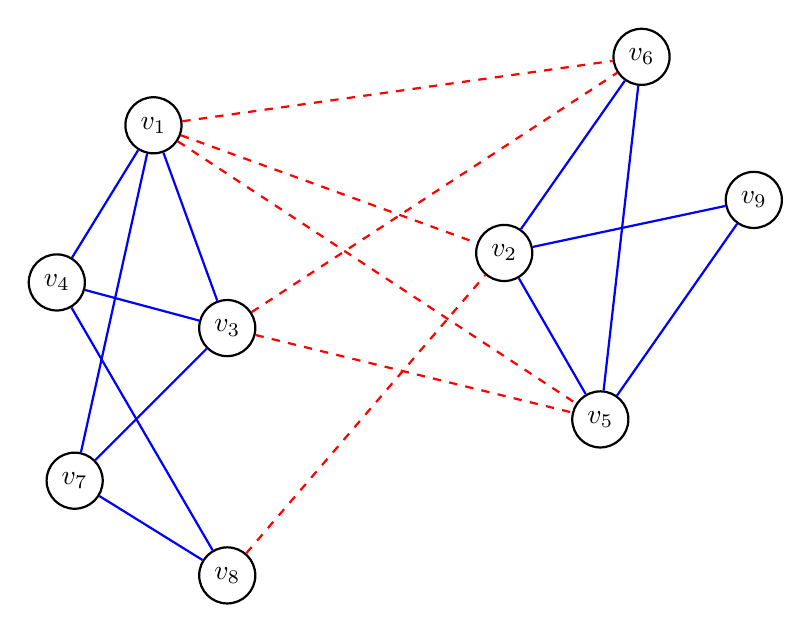
\begin{tikzpicture}

    \begin{scope}[every node/.style={circle,thick,draw}]
        \node (v1) at (0,0) {$v_1$};
        \node[position=-20:4cm from v1] (v2) {$v_2$};
        \node[position=-60:1.7cm from v2] (v5) {$v_5$};
        \node[position=55:2.3cm from v2] (v6) {$v_6$};
        \node[position=12:2.5cm from v2] (v9) {$v_9$};
        \node[position=-70:2cm from v1] (v3) {$v_3$};
        \node[position=-195:1.5cm from v3] (v4) {$v_4$};
        \node[position=225:2cm from v3] (v7) {$v_7$};
        \node[position=-90:2.4cm from v3] (v8) {$v_8$};
    \end{scope}

    % positive edges
    \begin{scope}[every edge/.style={thick,draw,blue},
        every node/.style={fill=white,circle}]
        % \draw (v4) -- (v1) -- (v3) -- (v2) -- (v1);
        \path 
        (v2) edge (v5) 
        (v5) edge (v9)
        (v2) edge (v6)
        (v6) edge (v5)
        (v2) edge (v9)      
        (v1) edge (v3)
        (v1) edge (v4)
        (v4) edge (v3)
        (v3) edge (v7)
        (v7) edge (v1)
        (v4) edge (v8)
        (v8) edge (v7)
        ;
    \end{scope}
    % negative edges
    \begin{scope}[every edge/.style={thick,draw,red,dashed},
        every node/.style={fill=white,circle}]
        % \draw (v4) -- (v1) -- (v3) -- (v2) -- (v1);
        \path 
        (v1) edge (v2)
        (v1) edge (v6)
        (v3) edge (v6)
        (v3) edge (v5)
        (v8) edge (v2)
        (v1) edge (v5)
        ;
    \end{scope}
  \end{tikzpicture}
  
    \caption{ A balanced signed graph. Solid blue edges are positive and dashed red edges are negative. Every cycle in this graph contains an even number of negative edges.}
    \label{fig:balanced-graph}
\end{figure}

The signed Laplacian matrix $\overline{L}$ of a signed graph $G$ is always positive-semidefinite and $\overline{L}$ is positive-definite iff $G$ is \textit{unbalanced} \cite{kunegis2010spectral,hou2005bounds,zaslavsky1982signed}. If the smallest eigenvalue of a graph $G$ is denoted by $\lambda_{1}(G)$, then $G$ is balanced iff $\lambda_{1}(G)=0$. Hou \cite{hou2005bounds} provides bounds on the value of $\lambda_{1}(G)$ which means that we can use the term as a measure of amount of imbalance in the signed graph $G$.

\subsection{Status Theory}
\label{sec:status-theory}
Guha et al. \cite{guha2004propagation} mention implicitly that a signed edge from $u$ to $v$ can be interpreted in a asymmetric manner different from "friend" or "enemy". Leskovec et al. \cite{leskovec2010signed,leskovec2010predicting} introduce the concept of \textit{status} to contextualize directed singed edges. A positive edge $u \xrightarrow{+} v$ indicates that $v$ has a higher status than $u$ and a negative edge $u \xrightarrow{-} v$ means that $v$ has a lower status than $u$. This concept of relative status can be propagated transitively along multiple steps which might lead to contradictions with balance theory \cite{leskovec2010signed}.

Given three vertices $v_1,v_2$ and $v_3$, the presence of an edge $v_1 \xrightarrow{+} v_2$ indicates that $v_1$ thinks $v_2$ has higher status, the edge $v_2 \xrightarrow{+} v_3$ indicates that $v_2$ thinks $v_3$ has higher status. Now we wish to to close this triad with an edge from $v_3$ to $v_1$. Status theory would say that through transitivity $v_1$ has lower status than $v_3$, therefore the prediction is $v_3 \xrightarrow{-} v_1$. Whereas, in balance theory we would predict a positive edge $v_3 \xrightarrow{+} v_1$ to make the cycle have even number of negative edges. This example can be seen in triads $S_1$ and $S_2$ shown in Figure~\ref{fig:status-triads}.

There are also cases when status theory is ambivalent to the edge that closes a triad. Consider the example when we have the edges $v_1 \xrightarrow{+} v_2$ and $v_2 \xrightarrow{-} v_3$. If we were to indicate the status of a vertex $v$ using the function $s(v)$, then the edges describe the following : $s(v_2)>s(v_1) $ and $s(v_2)>s(v_3)$. Therefore, we have no knowledge of the relative difference in status between the vertices $v_1$ and $v_3$. Hence, both edges $v_3 \xrightarrow{+} v_1$ ($s(v_3) > s(v_1)$) and $v_3 \xrightarrow{-} v_1$ ($s(v_1) > s(v_3)$) are equally valid for status theory. Balance theory on the other hand can only predict $v_3 \xrightarrow{-} v_1$ to keep the triad balanced. This case is shown in Figure~\ref{fig:status-triads} as triads $S_3$ and $S_4$.

\begin{figure}[!ht] 
    \centering
    \tikzset{
    position/.style args={#1:#2 from #3}{
        at=(#3.#1), anchor=#1+180, shift=(#1:#2)
    }
}

\begin{tikzpicture}

    \begin{scope}[every node/.style={circle,thick,draw}]
        \node (v2) at (0,0) {$v_2$};
        \node[position=-120:1cm from v2] (v1) {$v_1$};
        \node[position=-60:1cm from v2] (v3) {$v_3$};
        
        \node[right=2.5cm of v2] (v5) {$v_2$};
        \node[position=-120:1cm from v5] (v4) {$v_1$};
        \node[position=-60:1cm from v5] (v6) {$v_3$};
        
        \node[right=2.5cm of v5] (v8) {$v_2$};
        \node[position=-120:1cm from v8] (v7) {$v_1$};
        \node[position=-60:1cm from v8] (v9) {$v_3$};
        
        \node[right=2.5cm of v8] (v11) {$v_2$};
        \node[position=-120:1cm from v11] (v10) {$v_1$};
        \node[position=-60:1cm from v11] (v12) {$v_3$};
        

    \end{scope}

    \begin{scope}[>={Stealth[black]},
        positive/.style={thick,draw,->},
        negative/.style={thick,dashed,draw,->},
        every node/.style={fill=white,circle}]
        % \draw (v4) -- (v1) -- (v3) -- (v2) -- (v1);
        \path 
        (v1) edge[positive] node[above left=0.1mm and 0.1mm] {$+$} (v2)
        (v2) edge[positive] node[above right=0.1mm and 0.1mm] {$+$} (v3) 
        (v3) edge[positive] node[below] {$+$} node[below=1cm] {$S_1$}  (v1)      
        ;
        \path 
        (v4) edge[positive] node[above left=0.1mm and 0.1mm] {$+$} (v5)
        (v5) edge[positive] node[above right=0.1mm and 0.1mm] {$+$} (v6) 
        (v6) edge[negative] node[below] {$-$} node[below=1cm] {$S_2$}  (v4)      
        ;
        \path 
        (v7) edge[positive] node[above left=0.1mm and 0.1mm] {$+$} (v8)
        (v8) edge[negative] node[above right=0.1mm and 0.1mm] {$-$} (v9) 
        (v9) edge[negative] node[below] {$-$} node[below=1cm] {$S_3$}  (v7)      
        ;
        \path 
        (v10) edge[positive] node[above left=0.1mm and 0.1mm] {$+$} (v11)
        (v11) edge[negative] node[above right=0.1mm and 0.1mm] {$-$} (v12) 
        (v12) edge[positive] node[below] {$+$} node[below=1cm] {$S_4$}  (v10)      
        ;
    \end{scope}
  \end{tikzpicture}
  
    \caption{Triads in directed signed graphs. Triads $S_2,S_3$ and $S_4$ are compliant with status theory. Only triads $S_1$ and $S_3$ are compliant with balance theory.}
    \label{fig:status-triads}
\end{figure}

Each positive link inwards ($\indegree^{+}(v)$) and negative link outwards ($\outdegree^{-}(v)$) increases status. Each positive link outwards ($\outdegree^{+}(v)$) and negative link inwards ($\indegree^{-}(v)$) decreases status. Therefore, $\sigma(v) = \indegree^{+}(v) + \outdegree^{-}(v) - \outdegree^{+}(v)- \indegree^{-}(v)$ is a heuristic for the status of a node \cite{leskovec2010predicting}. An interesting fact is that the edge $u \xrightarrow{-} v$ can be converted into positive edge in the opposite direction $u \xleftarrow{+} v$. This fact reduces the number of unique triads that can be formed using status theory and will be used in edge prediction tasks that will be discussed in coming chapters.

\section{Hierarchy in directed networks}
\label{sec:hierarchy}
\begin{itemize}
    \item Discuss the hierarchy in DAGs
    \item Explain concept of Agony
    \item Provide existing algorithms to find the ranking of nodes.
\end{itemize}